% Provenance (never printed): see sources/outline_sources.md (Year 3: Gibbs
% energy and the phase rule in rocks, chemical potential recalled from the
% chemistry book; ternary diagrams; pseudosections, principle). Brief:
% sources/book5/BRIEFS.md, ch. 11. Curves from figdata/bachelor-3/
% gasp_tables.py, schreinemakers.py and regular_solution.py. Exercise and
% problem values in the Book 5 scratch calculator calc/ch11.py.
\chapter{Thermodynamique des roches}\label{ch:b3:petrological-thermodynamics}

Un grenat de quelques millimètres de diamètre a crû zone après zone pendant que son schiste était enfoui
et chauffé. Sa bordure conserve encore, dans ses teneurs en calcium, en fer et en magnésium,
le dernier équilibre atteint avec la biotite et le plagioclase qui l'entourent. Le
volume de deuxième année convertissait de telles compositions en une température et une pression
à l'aide de deux équations calibrées. Ce chapitre ouvre la boîte~: d'où viennent les
équations, jusqu'à quel point les tables d'enthalpies et d'entropies mesurées sont fiables,
combien de minéraux une roche peut contenir, comment les solutions solides se mélangent et
se démélangent, et comment un ordinateur transforme une composition globale en carte des
assemblages qu'elle doit montrer.

\begin{recall}
L'énergie de Gibbs, le potentiel chimique, l'activité et la constante d'équilibre,
la variance et la règle des phases, la lacune de miscibilité et la règle des
segments sont dans les volumes de chimie. La réaction univariante,
sa pente de Clapeyron $\Delta_rS/\Delta_rV$, le point invariant et le
diagramme des alumino-silicates calculé à partir des tables sont dans le volume de deuxième année, dans son
chapitre sur les faciès métamorphiques~; le géothermomètre et le géobaromètre, le
thermomètre d'échange grenat--biotite et le géobaromètre GASP, dans son chapitre sur
chemins P--T--t~; les diagrammes ternaires et la courbe cotectique, dans son chapitre sur les magmas. Une
solution solide et ses pôles purs sont dans le volume de première année, dans son chapitre sur
les minéraux.
\end{recall}

\section{Équilibre à partir des tables}\label{sec:b3:petrological-thermodynamics:tables}

Pour une réaction entre minéraux de composition fixée, l'équilibre à la
température $T$ et pression $P$ est $\Delta_rG(T, P) = 0$. Les tables donnent, à
\qty{298.15}{K} et \qty{1}{bar}, l'enthalpie de formation, l'entropie et
le volume molaire de chaque minéral, et la capacité calorifique $C_p(T)$ ci-dessus. Le
volume de deuxième année traitait $\Delta_rH$, $\Delta_rS$ et $\Delta_rV$ comme des constantes. Le
résultat général est le suivant.

\begin{theorem}[Énergie de Gibbs d'une réaction à $T$ et $P$]\label{thm:b3:petrological-thermodynamics:dg}
Soit une réaction ayant, à $T_0 = \qty{298.15}{K}$ et \qty{1}{bar}, une
enthalpie $\Delta_rH^\circ$ et entropie $\Delta_rS^\circ$, la variation de capacité
calorifique $\Delta_rC_p(T)$ et, pour les solides, une variation de volume $\Delta_rV$
indépendante de $T$ et de $P$. Alors
\[
  \Delta_rG(T, P) = \Delta_rH^\circ + \int_{T_0}^{T}\Delta_rC_p\,\mathrm dT
  - T\Bigl(\Delta_rS^\circ + \int_{T_0}^{T}\frac{\Delta_rC_p}{T}\,\mathrm dT\Bigr)
  + (P - 1)\,\Delta_rV ,
\]
et la droite d'équilibre est $P = 1 - \Delta_rG(T, 1)/\Delta_rV$.
\end{theorem}

\begin{proof}
À \qty{1}{bar}, $(\partial\Delta_rH/\partial T)_P = \Delta_rC_p$ et
$(\partial\Delta_rS/\partial T)_P = \Delta_rC_p/T$~; en intégrant depuis $T_0$
on obtient $\Delta_rH(T)$ et $\Delta_rS(T)$, puis $\Delta_rG = \Delta_rH -
T\Delta_rS$. À $T$ fixé, $(\partial\Delta_rG/\partial P)_T = \Delta_rV$,
constante par hypothèse~; en intégrant de 1 à $P$, on ajoute $(P - 1)\Delta_rV$.
En posant $\Delta_rG(T, P) = 0$, on obtient la droite.
\end{proof}

Les deux intégrales se compensent en partie~: leur somme vaut $\int_{T_0}^T\Delta_rC_p(1 -
T/T')\,\mathrm dT'$, le facteur $1 - T/T'$ étant négatif et petit
là où $T'$ est proche de $T$. Pour les solides, $\Delta_rC_p$ est lui-même faible,
car la capacité calorifique d'un minéral est presque la somme de celles de ses
oxydes. L'approximation à propriétés constantes est donc bonne, et les
tables indiquent à quel point elle l'est. Pour la réaction GASP,
\[
  \ce{3 CaAl2Si2O8 <=> Ca3Al2Si3O12 + 2 Al2SiO5 + SiO2},
\]
le tableau récapitulatif donne $\Delta_rH^\circ = \qty{-36.3}{kJ}$,
$\Delta_rS^\circ = \qty{-130.7}{J.K^{-1}}$ et $\Delta_rV =
\qty{-6.61}{J.bar^{-1}}$, soit une droite de pente \qty{19.8}{bar/K}~; les
tables à haute température, qui incluent les capacités calorifiques, donnent
$\Delta_rG$ tous les \qty{100}{K}, et les deux droites diffèrent de moins de
\qty{0.12}{kbar} jusqu'à \qty{1200}{K} (voir la figure ci-dessous).
% ledger: rh95:gasp-298, rh95:gasp-ht

Les expériences s'accordent moins bien. La réaction, inversée dans une presse à piston-cylindre entre
900 et \qty{1250}{\celsius}, la réaction se situe \qty{0.9}{kbar} plus haut que les
tables à \qty{627}{\celsius} et \qty{1.9}{kbar} plus haut à
\qty{927}{\celsius}. Avec $\Delta_rV = \qty{-6.61}{J.bar^{-1}}$,
\qty{1.9}{kbar} correspond à une erreur de \qty{12.6}{kJ} sur $\Delta_rH$~; les
incertitudes sur les quatre enthalpies de formation, \qty{3.2}{kJ} pour
grossulaire, \qty{2.0}{kJ} pour l'anorthite et la disthène, \qty{1.0}{kJ} pour
le quartz, se combinent pour donner environ \qty{8}{kJ} sur $\Delta_rH$. La calorimétrie fixe chaque
minéral à quelques kilojoules près~; une réaction portant sur de grandes unités formulaires multiplie
ces erreurs et les divise par une faible variation de volume.
% ledger: rh95:gasp-298, kn88:gasp

\begin{definition}[Base de données thermodynamiques à cohérence interne]\label{def:b3:petrological-thermodynamics:dataset}
Une \emph{base de données thermodynamiques à cohérence interne}\index{base de données thermodynamiques à cohérence interne}
est un tableau des propriétés standard de
nombreux minéraux et fluides (enthalpie de formation, entropie, volume, capacité
calorifique, dilatation thermique et compressibilité) ajustées ensemble, dans les
marges d'incertitude de la calorimétrie, de sorte que tout équilibre calculé à partir d'elle
reproduise les expériences inversées sur lesquelles elle a été ajustée.
\end{definition}

Une telle base est ajustée une seule fois, par moindres carrés pondérés ou par
programmation linéaire sur toutes les contraintes expérimentales à la fois, puis utilisée pour toute
réaction entre ses minéraux, y compris des réactions jamais étudiées en
laboratoire. Ses nombres ne sont pas des mesures indépendantes~: une enthalpie peut
être décalée d'un kilojoule pour ajuster une réaction à laquelle elle participe. Les valeurs issues
de bases différentes ne doivent jamais être mélangées.

\begin{omfigure}
\begin{tikzpicture}
\begin{axis}[omrecord, width=0.78\linewidth, height=0.5\linewidth,
  xlabel={température (\unit{\celsius})}, ylabel={pression (\unit{kbar})},
  xmin=400, xmax=1300, ymin=0, ymax=30, legend style={font=\scriptsize,
  at={(0.03,0.97)}, anchor=north west, legend cell align=left}]
% computed in figdata/bachelor-3/gasp_tables.py
\fill[omLithLime!60] (axis cs:900,19) rectangle (axis cs:1250,28);
\addplot[red!70!black, very thick] table[x=tc, y=p_kn88] {figdata/out/bachelor-3-gasp_tables-lines.dat};
\addlegendentry{expérience (pôles purs)}
\addplot[omDef, thick, densely dashed] table[x=tc, y=p_const] {figdata/out/bachelor-3-gasp_tables-lines.dat};
\addlegendentry{tables, $\Delta_rH$ et $\Delta_rS$ constants}
\addplot[omDef, only marks, mark=*, mark size=1.8pt] table[x=tc, y=p_table] {figdata/out/bachelor-3-gasp_tables-tables.dat};
\addlegendentry{tables, avec capacités calorifiques}
\node[font=\scriptsize, align=center] at (axis cs:1075,26.3) {expériences\\inversées};
\node[font=\scriptsize] at (axis cs:560,4) {anorthite};
\node[font=\scriptsize, align=center] at (axis cs:560,17) {grossulaire + disthène\\+ quartz};
\end{axis}
\end{tikzpicture}

\par\smallskip{\small La réaction GASP des pôles purs, 3 anorthite = grossulaire +
2 disthène + quartz, calculée à partir des tables calorimétriques, avec des
propriétés constantes (tirets) et avec les capacités calorifiques (points), et la droite ajustée
aux expériences inversées réalisées dans la zone ombrée (en rouge, extrapolée sous
\qty{900}{\celsius}).}\label{fig:b3:petrological-thermodynamics:gasp}
\end{omfigure}
% ledger: rh95:gasp-298, rh95:gasp-ht, kn88:gasp

\section{La règle des phases dans les roches}\label{sec:b3:petrological-thermodynamics:phase-rule}

La règle des phases de la chimie donne la variance $F = c - p + 2$ d'un système de
$c$ constituants dans $p$ phases. Une roche est un tel système, et ses minéraux montrent
dans quelle partie du plan pression--température elle a atteint l'équilibre.

\begin{proposition}[Règle des phases minéralogique]\label{prop:b3:petrological-thermodynamics:goldschmidt}
Une roche qui a atteint l'équilibre à une pression et une température choisies
librement dans une région du plan pression--température compte au plus autant de
phases que de constituants~: $p \le c$. Il s'agit de la
\emph{règle des phases minéralogique}\index{règle des phases minéralogique}.
\end{proposition}

\begin{proof}
La règle des phases donne $F = c - p + 2$ variables intensives indépendantes. Si la
pression et la température peuvent varier toutes deux sans modifier l'assemblage, deux
d'entre elles sont libres~: $F \ge 2$, donc $p \le c$. Une roche avec $p = c + 1$ phases
se trouve sur une droite univariante~; avec $p = c + 2$, sur un point invariant~; aucun des deux
n'est probable pour une roche prélevée au hasard.
\end{proof}

Une roche qui enfreint la règle a soit atteint l'équilibre sur une droite de réaction,
que ses textures peuvent révéler, soit n'a jamais atteint l'équilibre dans son ensemble~: les textures en couronne,
les minéraux zonés et les grains reliques sont des causes fréquentes. Compter les
constituants demande du soin. Un constituant présent seulement dans une phase de composition fixe, comme
le zircon, peut être retiré avec sa phase~; un constituant fixé par un réservoir extérieur
comme l'eau lorsqu'un fluide traverse la roche, n'est pas compté
comme libre, puisque son potentiel chimique est imposé.

Autour d'un point invariant, les droites univariantes ne se croisent pas au hasard. Dans un
système de $c$ constituants, $c + 2$ phases se rencontrent au point et $c + 2$
réactions rayonnent à partir de lui, chacune écrite parmi $c + 1$ phases et nommée d'après
la phase qu'elle omet, entre crochets.

\begin{definition}[Analyse de Schreinemakers]\label{def:b3:petrological-thermodynamics:schreinemakers}
L'\emph{analyse de Schreinemakers}\index{analyse de Schreinemakers} est la méthode
qui dispose les droites univariantes autour d'un point invariant à partir des
compositions des seules phases, avant toute mesure de leurs
propriétés thermodynamiques~: elle fixe l'ordre des droites, le côté de chaque
droite stable, et les assemblages de chaque secteur compris entre elles.
\end{definition}

\begin{method}[Règles de Schreinemakers]\label{met:b3:petrological-thermodynamics:schreinemakers}
(1) On écrit les $c + 2$ réactions, chacune en omettant une phase. (2) Chaque droite est
stable d'un côté du point et métastable de l'autre. (3) Le
prolongement métastable de la droite ($i$), qui omet la phase $i$, se situe dans un
secteur où $i$ est stable. (4) Aucun secteur compris entre deux droites stables consécutives
n'excède pas \ang{180}. (5) De part et d'autre d'une droite, les assemblages
de chaque côté sont ceux des deux membres de sa réaction. Fixer une seule droite avec des données
fixe alors tout le faisceau, à une image miroir près.
\end{method}

Le point triple des alumino-silicates du volume de deuxième année est le cas le plus simple,
$c = 1$ et trois droites. La figure ci-dessous présente un cas à deux constituants
calculé par \omterm{def:b3:petrological-thermodynamics:minimisation}{minimisation de l'énergie de Gibbs} en chaque point.

\begin{omfigure}
\begin{tikzpicture}
\begin{axis}[omrecord, width=0.62\linewidth, height=0.5\linewidth,
  xlabel={température (\unit{\celsius})}, ylabel={pression (\unit{kbar})},
  xmin=400, xmax=800, ymin=1, ymax=9, grid=none]
% computed in figdata/bachelor-3/schreinemakers.py
\addplot[omDef, very thick] table[x=t, y=p] {figdata/out/bachelor-3-schreinemakers-ray_A_s.dat};
\addplot[omDef, thick, densely dashed] table[x=t, y=p] {figdata/out/bachelor-3-schreinemakers-ray_A_m.dat};
\addplot[omDef, very thick] table[x=t, y=p] {figdata/out/bachelor-3-schreinemakers-ray_B_s.dat};
\addplot[omDef, thick, densely dashed] table[x=t, y=p] {figdata/out/bachelor-3-schreinemakers-ray_B_m.dat};
\addplot[omDef, very thick] table[x=t, y=p] {figdata/out/bachelor-3-schreinemakers-ray_C_s.dat};
\addplot[omDef, thick, densely dashed] table[x=t, y=p] {figdata/out/bachelor-3-schreinemakers-ray_C_m.dat};
\addplot[omDef, very thick] table[x=t, y=p] {figdata/out/bachelor-3-schreinemakers-ray_D_s.dat};
\addplot[omDef, thick, densely dashed] table[x=t, y=p] {figdata/out/bachelor-3-schreinemakers-ray_D_m.dat};
\node[font=\scriptsize, fill=white, inner sep=1pt] at (axis cs:740,7.85) {(A)};
\node[font=\scriptsize, fill=white, inner sep=1pt] at (axis cs:540,8.75) {(C)};
\node[font=\scriptsize, fill=white, inner sep=1pt] at (axis cs:540,1.6) {(B)};
\node[font=\scriptsize, fill=white, inner sep=1pt] at (axis cs:740,2.15) {(D)};
\node[font=\scriptsize, align=center] at (axis cs:592,7.7) {A + B\\B + D};
\node[font=\scriptsize, align=center] at (axis cs:450,5.0) {A + D};
\node[font=\scriptsize, align=center] at (axis cs:592,2.4) {A + C\\C + D};
\node[font=\scriptsize, align=center] at (axis cs:765,5.0) {A + B\\B + C\\C + D};
\end{axis}
\end{tikzpicture}

\par\smallskip{\small Un faisceau de Schreinemakers dans un système à deux constituants avec
quatre phases de compositions A (0), B ($1/3$), C ($2/3$) et D (1),
calculé pour des propriétés fictives~: droites stables en trait plein, prolongements
métastables en tirets, et les paires stables de chaque secteur. (D) est A + C = 2B, (A) est B + D =
2C, (C) est 2A + D = 3B et (B) est A + 2D = 3C.}\label{fig:b3:petrological-thermodynamics:schreinemakers}
\end{omfigure}

\section{Solutions solides}\label{sec:b3:petrological-thermodynamics:solutions}

La plupart des minéraux formant les roches sont des solutions solides, et leurs pôles purs
apparaissent dans les réactions par l'intermédiaire de leurs activités. Le volume de deuxième année a pris $a = X^3$ pour
le grossulaire dans un grenat et $a = X$ pour l'anorthite dans un plagioclase.
Les deux relèvent d'un même modèle.

\begin{definition}[Modèle d'activité par mélange sur sites]\label{def:b3:petrological-thermodynamics:site-mixing}
Dans un \emph{modèle d'activité par mélange sur sites}\index{modèle d'activité par mélange sur sites}, les
ions d'un minéral se mélangent au hasard sur chaque site cristallographique, indépendamment
des autres sites. L'activité idéale d'un pôle pur est alors le produit,
sur les sites, de la fraction de chaque site qu'il occupe, élevée à la puissance
égale au nombre de tels sites par formule unitaire~: $a_i = \prod_s X_{s,i}^{\,n_s}$.
\end{definition}

Un grenat $X_3Y_2\ce{Si3O12}$ possède trois sites dodécaédriques $X$ occupés par
\ce{Ca}, \ce{Fe}, \ce{Mg} et \ce{Mn}~: $a_{\text{grossulaire}} =
X_{\text{Ca}}^3$. Un grenat avec $X_{\text{Ca}} = 0.10$ renferme
\qty{10}{\percent} de grossulaire, mais son activité vaut $10^{-3}$. Le
modèle idéal dénombre les configurations~; les solutions réelles ont aussi une énergie d'excès,
car des ions de tailles différentes contraignent le réseau.

\begin{definition}[Diagramme énergie de Gibbs--composition]\label{def:b3:petrological-thermodynamics:gx}
Un \emph{diagramme énergie de Gibbs--composition}\index{diagramme énergie de Gibbs--composition}
représente, à température et pression fixées, l'énergie de Gibbs molaire de
chaque phase d'un système en fonction de sa composition. L'assemblage stable
d'une composition globale quelconque se situe sur l'enveloppe convexe inférieure des courbes~:
une seule phase lorsque sa courbe appartient à l'enveloppe, deux phases aux extrémités d'une tangente commune.
\end{definition}

\begin{proposition}[Solution régulière]\label{prop:b3:petrological-thermodynamics:regular}
Dans une solution binaire comportant un site de mélange par formule unitaire et
une énergie d'interaction $W$, l'énergie de Gibbs de mélange s'écrit
\[
  G_{\text{mix}} = RT\bigl[x\ln x + (1 - x)\ln(1 - x)\bigr] + Wx(1 - x).
\]
Si $W > 0$, la solution est stable à toute composition au-dessus de $T_c =
W/(2R)$~; en dessous de $T_c$, la courbe présente deux points d'inflexion et
les compositions comprises entre les deux points de sa tangente commune se séparent en deux phases.
\end{proposition}

\begin{proof}
Le premier terme vaut $-T$ fois l'entropie configurationnelle du mélange aléatoire~;
le second, l'énergie d'excès la plus simple, symétrique et nulle aux deux extrémités.
En dérivant deux fois, $G''_{\text{mix}} = RT/[x(1 - x)] - 2W$. Son minimum
sur $x$ est atteint en $x = 1/2$, où il vaut $4RT - 2W$, qui est positif pour
tout $x$ si $T > W/(2R)$. En dessous, $G''_{\text{mix}} < 0$ sur un intervalle
autour de $1/2$~: la courbe s'infléchit vers le bas à cet endroit, une droite joignant deux points
de la courbe passe sous elle, et, selon la définition précédente, la roche
est constituée de deux phases.
\end{proof}

\begin{definition}[Solvus et exsolution]\label{def:b3:petrological-thermodynamics:solvus}
Le \emph{solvus}\index{solvus} est la courbe, dans le plan température--composition,
qui délimite la lacune de miscibilité d'une solution solide~: en dessous, un
cristal unique de composition intermédiaire est instable et se scinde en deux.
L'\emph{exsolution}\index{exsolution (minéral)} désigne cette
séparation au sein d'un cristal lors du refroidissement~: des lamelles d'une
composition croissent dans un hôte de l'autre.
\end{definition}

Les feldspaths alcalins, les pyroxènes et les amphiboles présentent des lamelles
d'\omterm{def:b3:petrological-thermodynamics:solvus}{exsolution}, visibles au microscope ou à l'œil nu~: la perthite de nombreux
granites est un feldspath alcalin exsolvé, un hôte riche en potassium contenant
des lamelles riches en sodium. Entre le \omterm{def:b3:petrological-thermodynamics:solvus}{solvus} et la spinodale, où $G''_{\text{mix}} = 0$,
un cristal doit d'abord faire germer la seconde phase~; à l'intérieur de la
spinodale, toute petite fluctuation de composition croît par diffusion seule.

\begin{omfigure}
\begin{tikzpicture}
\begin{groupplot}[group style={group size=2 by 1, horizontal sep=1.7cm},
  omrecord, width=0.47\linewidth, height=0.42\linewidth, title style={font=\small},
  legend style={font=\scriptsize, legend cell align=left}]
\nextgroupplot[title={(a) énergie de Gibbs de mélange}, xlabel={$x$},
  ylabel={$G_{\text{mix}}$ (\unit{kJ.mol^{-1}})}, xmin=0, xmax=1, ymin=-9, ymax=1,
  legend style={at={(0.5,0.03)}, anchor=south}]
% computed in figdata/bachelor-3/regular_solution.py
\addplot[black, thick, densely dotted] table[x=x, y=g1500] {figdata/out/bachelor-3-regular_solution-gx.dat};
\addlegendentry{\qty{1500}{K}}
\addplot[red!70!black, thick, densely dashed] table[x=x, y=g1203] {figdata/out/bachelor-3-regular_solution-gx.dat};
\addlegendentry{$T_c = \qty{1203}{K}$}
\addplot[omDef, thick] table[x=x, y=g0900] {figdata/out/bachelor-3-regular_solution-gx.dat};
\addlegendentry{\qty{900}{K}}
\addplot[omDef, thin, forget plot] coordinates {(0.111,-0.635) (0.889,-0.635)};
\nextgroupplot[title={(b) solvus et section à $X_0 = 0.3$}, xlabel={$x$},
  ylabel={température (\unit{K})}, xmin=0, xmax=1, ymin=600, ymax=1300,
  legend style={at={(0.5,0.03)}, anchor=south}]
\addplot[omDef, thick] table[x=x, y=t_bin] {figdata/out/bachelor-3-regular_solution-solvus.dat};
\addlegendentry{solvus}
\addplot[black, thick, densely dotted] table[x=x, y=t_spin] {figdata/out/bachelor-3-regular_solution-solvus.dat};
\addlegendentry{spinodale}
\addplot[red!70!black, thick, forget plot] coordinates {(0.3,600) (0.3,1300)};
\addplot[red!70!black, thick, densely dashed] table[x=x2, y=t] {figdata/out/bachelor-3-regular_solution-section.dat};
\addlegendentry{isoplèthes à $X_0$}
\addplot[red!70!black, thick, densely dashed, forget plot] table[x=x1, y=t] {figdata/out/bachelor-3-regular_solution-section.dat};
\node[font=\scriptsize] at (axis cs:0.5,1250) {une phase};
\node[font=\scriptsize] at (axis cs:0.5,950) {deux phases};
\end{groupplot}
\end{tikzpicture}

\par\smallskip{\small Une solution régulière avec $W = \qty{20}{kJ.mol^{-1}}$
(à titre illustratif). (a) Énergie de Gibbs de mélange à trois températures~; à
\qty{900}{K}, la tangente commune (trait fin) touche la courbe en $x = 0.11$
et 0.89. (b) Le \omterm{def:b3:petrological-thermodynamics:solvus}{solvus} et la spinodale~; une roche de composition globale $X_0 =
0.3$ (trait rouge vertical) est monophasée au-dessus de \qty{1136}{K} et
biphasée en dessous, dont les compositions suivent le \omterm{def:b3:petrological-thermodynamics:solvus}{solvus} (tirets).}\label{fig:b3:petrological-thermodynamics:solvus}
\end{omfigure}

\section{Pseudosections}\label{sec:b3:petrological-thermodynamics:pseudosections}

Le panneau (b) de la figure précédente est déjà une petite \omterm{def:b3:petrological-thermodynamics:pseudosection}{pseudosection}~: pour une
composition globale donnée, il indique quelles phases sont stables à chaque
température, ainsi que leurs compositions et leurs proportions. Une roche
métamorphique compte une dizaine de composants et de nombreuses solutions solides, mais le principe reste le même.

\begin{definition}[Minimisation de l'énergie de Gibbs]\label{def:b3:petrological-thermodynamics:minimisation}
La \emph{minimisation de l'énergie de Gibbs}\index{minimisation de l'énergie de Gibbs} détermine, à
température et pression données, l'ensemble des phases, leurs compositions et
leurs quantités qui minimisent l'énergie de Gibbs totale d'un système de
composition globale fixée, sous la contrainte de conservation de chaque composant.
\end{definition}

\begin{definition}[Pseudosection, isoplèthe, composition globale effective]\label{def:b3:petrological-thermodynamics:pseudosection}
Une \emph{pseudosection}\index{pseudosection} est un diagramme de phases, généralement dans
le plan pression--température, calculé pour une composition globale fixée~: il
est découpé en domaines, chacun étiqueté par l'assemblage qui minimise
l'énergie de Gibbs à cet endroit. Une \emph{isoplèthe}\index{isoplèthe (pseudosection)}
est une ligne d'une pseudosection le long de laquelle une variable de composition
d'une phase, ou sa quantité, reste constante. La \emph{composition globale
effective}\index{composition globale effective} est la part de la composition de la roche qui
participe encore à l'équilibre, une fois ôtés les cœurs des cristaux
zonés, les porphyroblastes coupés de la matrice et les autres matériaux
isolés.
\end{definition}

Une \omterm{def:b3:petrological-thermodynamics:pseudosection}{pseudosection} ne montre pas de lignes univariantes au sens du volume de deuxième année~:
dans un système à solutions solides, la limite entre deux domaines est
là où une phase apparaît ou disparaît, et sa position dépend de la
composition globale. La lecture en est directe. L'assemblage observé fixe un domaine~;
la composition mesurée d'un minéral, la teneur en calcium du bord d'un grenat par
exemple, choisit une \omterm{def:b3:petrological-thermodynamics:pseudosection}{isoplèthe} à l'intérieur du domaine~; une seconde \omterm{def:b3:petrological-thermodynamics:pseudosection}{isoplèthe}, d'un autre élément
ou d'un autre minéral, la coupe à la pression et à la température de
l'équilibre. Les grenats zonés portent une suite de ces croisements, un pour chaque
zone, le long du chemin suivi par la roche. Mais, à mesure que le grenat croît, son cœur
retire du manganèse et du calcium à la portée de la matrice~: la
\omterm{def:b3:petrological-thermodynamics:pseudosection}{composition globale effective} change, et la \omterm{def:b3:petrological-thermodynamics:pseudosection}{pseudosection} doit être recalculée pour les
zones suivantes.

\begin{inthelab}[Le bureau du pétrologue]
\begin{minipage}[t]{0.55\linewidth}\vspace{0pt}
Le pétrologue examine d'abord une lame mince au microscope polarisant,
pour identifier l'assemblage, ses textures et les grains ayant crû
ensemble. La même lame, métallisée au carbone, passe ensuite à la
microsonde électronique, qui mesure la composition de points de quelques
micromètres de large le long de profils traversant les grenats. Un logiciel qui minimise l'énergie de Gibbs
avec une \omterm{def:b3:petrological-thermodynamics:dataset}{base de données thermodynamiques à cohérence interne} et un jeu de modèles d'activité calcule
une \omterm{def:b3:petrological-thermodynamics:pseudosection}{pseudosection} pour la composition globale, mesurée sur une tranche de la même
roche. Les \omterm{def:b3:petrological-thermodynamics:pseudosection}{isoplèthes} des compositions mesurées y sont reportées, et leur croisement
en fournit la réponse. C'est l'incertitude de la base de données et des modèles
d'activité, et non celle des mesures, qui limite en général la précision.
\end{minipage}\hfill
\begin{minipage}[t]{0.42\linewidth}\vspace{0pt}
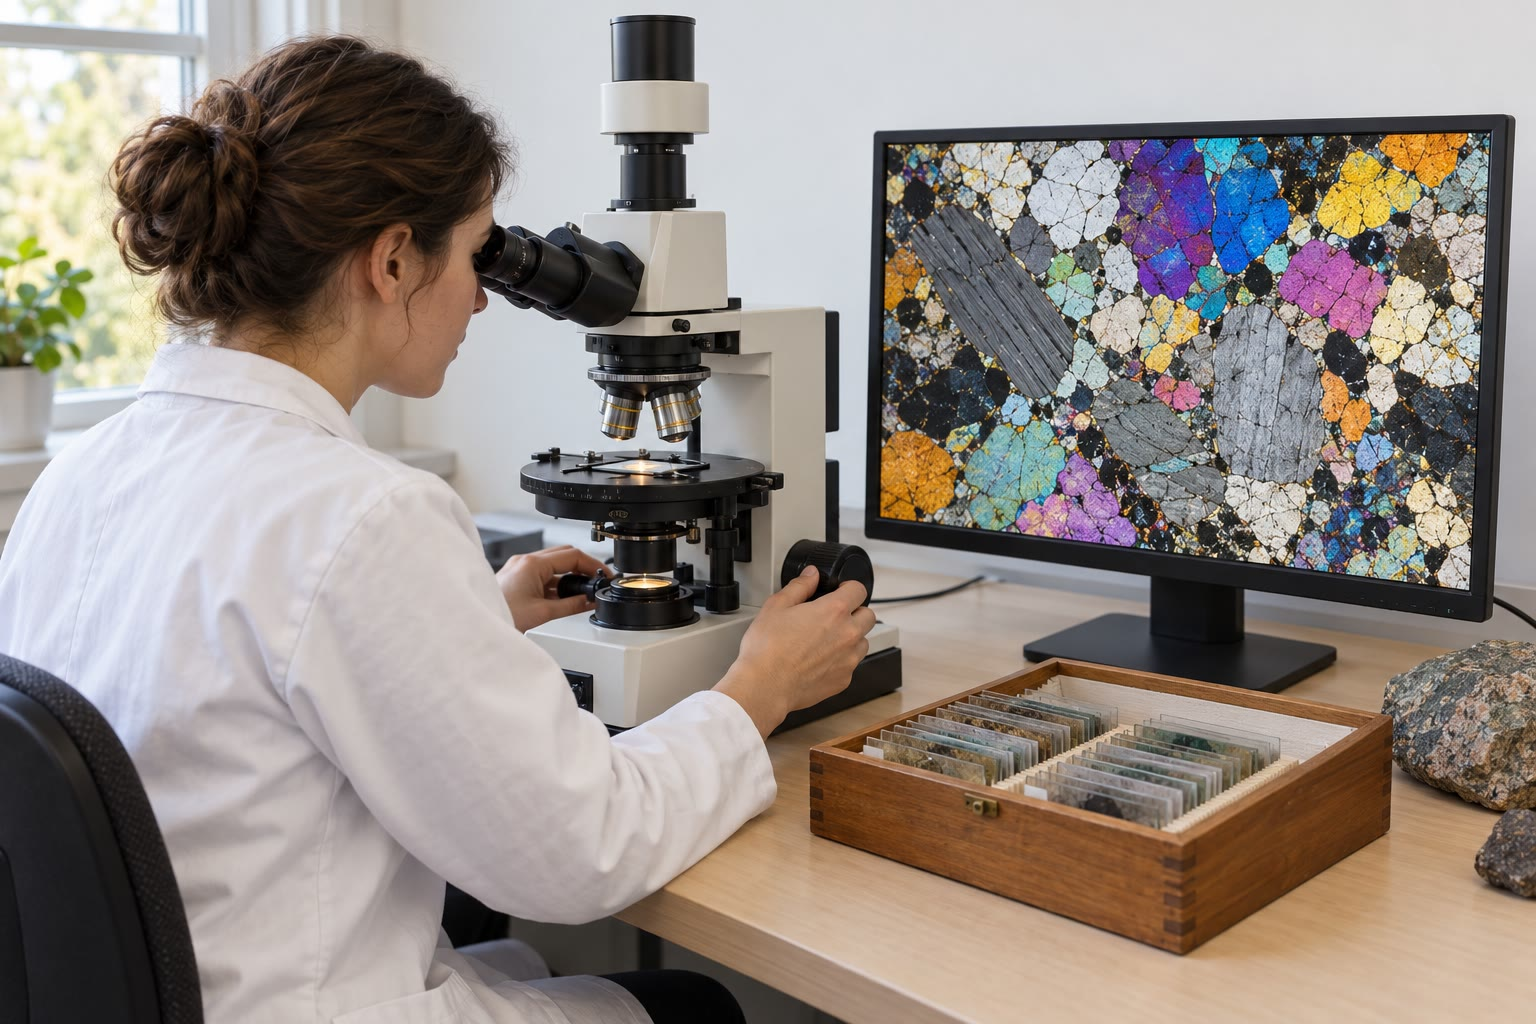
\includegraphics[width=\linewidth]{images/book5/ai/b3-petrology-desk.jpg}

{\scriptsize Un pétrologue devant un microscope polarisant, une boîte de lames
minces à portée de main et une lame mince en lumière polarisée sur l'écran
(Illustration générée par IA.)}
\end{minipage}
\end{inthelab}

\section{Exercices}

\begin{exercise}[$\star$]\label{exo:b3:petrological-thermodynamics:1}
D'après les tables, l'albite a $\Delta_fH^\circ = \qty{-3935.0}{kJ}$, $S^\circ =
\qty{207.4}{J.K^{-1}}$, $V = \qty{100.07}{cm^3}$~; la jadéite $-3029.3$, 133.5,
60.40~; le quartz $-910.7$, 41.5, 22.69 (par mole). Pour l'albite = jadéite + quartz,
calculer $\Delta_rH$, $\Delta_rS$, $\Delta_rV$ (en \unit{J.bar^{-1}}), la
pente de Clapeyron et la pression de la courbe à \qty{600}{\celsius} avec
des propriétés constantes.
\end{exercise}
% ledger: rh95:ab-jd-qz

\begin{exercise}[$\star$]\label{exo:b3:petrological-thermodynamics:2}
Une roche du système \ce{MgO}--\ce{SiO2} contient forstérite, enstatite et
quartz. Appliquer la \omterm{prop:b3:petrological-thermodynamics:goldschmidt}{règle des phases minéralogique}. Que conclure~?
\end{exercise}

\begin{exercise}[$\star$]\label{exo:b3:petrological-thermodynamics:3}
Calculer les activités idéales des pôles grossulaire et pyrope dans un grenat avec
$X_{\text{Ca}} = 0.20$ et $X_{\text{Mg}} = 0.15$, et celle de l'anorthite dans un
plagioclase avec $X_{\text{an}} = 0.40$ (un seul site).
\end{exercise}

\begin{exercise}[$\star$]\label{exo:b3:petrological-thermodynamics:4}
Calculer la température critique d'une solution régulière avec $W =
\qty{15}{kJ.mol^{-1}}$. Quelle valeur de $W$ donne $T_c = \qty{1000}{K}$~?
\end{exercise}

\begin{exercise}[$\star\star$]\label{exo:b3:petrological-thermodynamics:5}
À \qty{1000}{K}, les tables donnent les énergies de Gibbs de formation
$-5432.2$ (grossulaire), $-3478.1$ (anorthite), $-2088.8$ (disthène) et $-730.2$
(quartz), en \unit{kJ.mol^{-1}}. Calculer $\Delta_rG$ de la réaction GASP à
\qty{1}{bar}, puis la pression d'équilibre correspondante, et comparer avec la droite
expérimentale $P_0 = 22.80\,T - 1093$ (bar, \unit{\celsius}).
\end{exercise}
% ledger: rh95:gasp-ht, kn88:gasp

\begin{exercise}[$\star\star$]\label{exo:b3:petrological-thermodynamics:6}
Pour la solution régulière de la figure ($W = \qty{20}{kJ.mol^{-1}}$), calculer
$G_{\text{mix}}$ à $x = 0.5$ et \qty{900}{K}, puis au flanc du \omterm{def:b3:petrological-thermodynamics:solvus}{solvus} $x =
0.111$. Montrer que la séparation d'un cristal de composition 0.5 en ses deux flancs
abaisse son énergie de Gibbs, et de quelle quantité.
\end{exercise}

\begin{exercise}[$\star\star$]\label{exo:b3:petrological-thermodynamics:7}
Combien de phases se rejoignent en un point invariant, et combien de lignes univariantes
partent de celui-ci, dans un système à trois constituants~? Dans le faisceau de la
figure, vérifier que chacune des quatre réactions est équilibrée.
\end{exercise}

\begin{exercise}[$\star\star$]\label{exo:b3:petrological-thermodynamics:8}
Une roche de composition globale $X_0 = 0.3$ dans la solution régulière de la figure
s'est refroidie à \qty{900}{K}, où les flancs du \omterm{def:b3:petrological-thermodynamics:solvus}{solvus} valent 0.111 et 0.889.
Calculer la proportion de chaque phase.
\end{exercise}

\begin{exercise}[$\star\star$]\label{exo:b3:petrological-thermodynamics:9}
Avec le géobaromètre GASP $P = P_0 + (3RT/6.21)\ln(X_{\text{Ca}}/X_{\text{an}})$
(bar), calculer $\partial P/\partial X_{\text{an}}$ à \qty{900}{K} et
$X_{\text{an}} = 0.30$. De combien une erreur de 0.01 sur $X_{\text{an}}$
déplace la pression~?
\end{exercise}

\begin{exercise}[$\star\star\star$]\label{exo:b3:petrological-thermodynamics:10}
Montrer que la spinodale d'une solution régulière est $x(1 - x) = RT/(2W)$. À quelle
température un cristal de composition 0.3 devient-il instable à toute petite
fluctuation, pour $W = \qty{20}{kJ.mol^{-1}}$~? Comparer avec la température à
laquelle il atteint le \omterm{def:b3:petrological-thermodynamics:solvus}{solvus}, $T = W(1 - 2x)/[R\ln((1 - x)/x)]$, et expliquer
l'écart.
\end{exercise}

\begin{exercise}[$\star\star\star$]\label{exo:b3:petrological-thermodynamics:11}
Montrer que le \omterm{def:b3:petrological-thermodynamics:solvus}{solvus} d'une solution régulière symétrique vérifie $RT\ln[x/(1 -
x)] + W(1 - 2x) = 0$, et qu'il atteint son maximum, $T_c = W/(2R)$, en $x
= 1/2$.
\end{exercise}

\begin{exercise}[$\star\star\star$]\label{exo:b3:petrological-thermodynamics:12}
Une roche contient \qty{2.0}{wt\percent} \ce{MnO}. Les cœurs de grenat contenant
\qty{10}{wt\percent} \ce{MnO} représentent \qty{8}{wt\percent} de la roche et sont
isolés de la matrice. Calculer la teneur en \ce{MnO} de la \omterm{def:b3:petrological-thermodynamics:pseudosection}{composition globale
effective}. Pourquoi cela compte-t-il pour la \omterm{def:b3:petrological-thermodynamics:pseudosection}{pseudosection} des bords de grenat~?
\end{exercise}

\section{Problème~: le grenat du schiste de Varden}

\begin{problem}[{Problème du week-end --- la pression et la température d'un
schiste inventé, à partir de tables, de la règle des phases, des modèles d'activité et
thermobarométrie}]
\label{pb:b3:petrological-thermodynamics:1}
% values: calc/ch11.py; gasp_tables.py
Le schiste du socle de Varden Hills, métamorphisé il y a environ
\qty{480}{Ma}, contient du grenat, de la biotite, de la muscovite, du plagioclase, de la kyanite et
du quartz. Au bord d'un grenat et dans les grains qui l'entourent, la microsonde électronique
donne~: grenat $X_{\text{Fe}} = 0.74$, $X_{\text{Mg}} = 0.12$, $X_{\text{Ca}} =
0.10$, $X_{\text{Mn}} = 0.04$~; biotite $\ce{Mg}/(\ce{Mg} + \ce{Fe}) = 0.45$~;
plagioclase $X_{\text{an}} = 0.30$. Utiliser les tables de ce chapitre pour la
réaction GASP, le géothermomètre du volume de deuxième année
\[
T = \frac{52\,635 + 0.311P}{20.20 - 3R\ln K_D}\quad(T \text{ en K}, P
\text{ en bar}),
\]
et son géobaromètre expérimental $P = 22.80\,t - 1093 + (3RT/6.21)\ln
(X_{\text{Ca}}/X_{\text{an}})$, avec $t$ en \unit{\celsius} et $T$ en
kelvins. Prendre $R = \qty{8.314}{J.mol^{-1}.K^{-1}}$, une masse volumique crustale de
\qty{2800}{kg/m^3} et $g = \qty{9.81}{m/s^2}$.

\medskip\noindent\textbf{Partie I --- Les tables.}
\begin{enumerate}
  \item À partir du tableau récapitulatif, calculer $\Delta_rH^\circ$, $\Delta_rS^\circ$
        et $\Delta_rV$ de la réaction GASP.
  \item Calculer $\Delta_rG$ à \qty{298.15}{K} et \qty{1}{bar}. Quel côté
        est stable en surface~?
  \item Calculer la pression d'équilibre des pôles purs à \qty{900}{K} avec
        des propriétés constantes, et la pente de Clapeyron.
  \item Les tables haute température donnent $\Delta_rG = \qty{81.5}{kJ}$ à
        \qty{900}{K} et \qty{119.8}{kJ} à \qty{1200}{K} (\qty{1}{bar}).
        Calculer les pressions.
  \item Comparer avec la droite expérimentale aux mêmes températures.
  \item Quelle erreur sur $\Delta_rH$ expliquerait l'écart à \qty{1200}{K}~?
        Comparer avec l'incertitude combinée des quatre enthalpies.
  \item Pourquoi les capacités calorifiques modifient-elles si peu le résultat~?
\end{enumerate}

\medskip\noindent\textbf{Partie II --- La règle des phases.}
\begin{enumerate}[resume]
  \item Lister les constituants nécessaires pour décrire les six minéraux et un fluide
        aqueux, et compter les phases.
  \item Calculer la variance à l'aide de la règle des phases et vérifier la
        \omterm{prop:b3:petrological-thermodynamics:goldschmidt}{règle des phases minéralogique}.
  \item Un second échantillon renferme de la kyanite et de la sillimanite côte à côte. Que
        dit-il de sa pression et de sa température~?
  \item De l'eau a circulé dans la roche pendant le métamorphisme. Comment cela
        modifie-t-il le décompte~?
\end{enumerate}

\medskip\noindent\textbf{Partie III --- Activités et thermobarométrie.}
\begin{enumerate}[resume]
  \item Calculer les activités idéales du grossulaire et de l'anorthite, et $\ln K$
        de la réaction GASP dans la roche.
  \item Calculer $K_D$ de l'échange grenat--biotite.
  \item Calculer la température à \qty{8}{kbar}.
  \item Calculer la pression GASP à cette température.
  \item Itérer jusqu'à l'intersection des deux équations.
  \item Refaire l'intersection avec la droite des pôles purs des tables
        à la place de la droite expérimentale (avec $\Delta_rV = \qty{-6.61}{J.bar^{-1}}$).
        Quel résultat retenir, et pourquoi~?
  \item De combien une erreur de 0.05 sur $X_{\text{an}}$ déplace-t-elle le
        résultat~?
\end{enumerate}

\medskip\noindent\textbf{Partie IV --- L'enfouissement.}
\begin{enumerate}[resume]
  \item Avec les propriétés constantes du volume de deuxième année, la réaction kyanite =
        sillimanite a $\Delta_rH = \qty{7.7}{kJ}$, $\Delta_rS =
        \qty{12.6}{J.K^{-1}}$, $\Delta_rV = \qty{0.571}{J.bar^{-1}}$. Le résultat
        est-il dans le champ de la kyanite~?
  \item Calculer la profondeur d'enfouissement.
  \item Le cœur du grenat a $X_{\text{Ca}} = 0.07$ et s'est formé avec du plagioclase
        de même $X_{\text{an}}$, à peu près à la même température. Le cœur s'est-il
        formé plus profondément ou moins profondément que le bord~?
  \item Donner la pression maximale et la profondeur d'enfouissement du schiste de Varden.
\end{enumerate}
\end{problem}
